\documentclass[12pt]{article}
\usepackage{array}
\usepackage{amsmath}
\usepackage{mathtools}
\usepackage{gensymb}
\usepackage{graphicx}
\usepackage{float}
\usepackage{caption}
\usepackage{setspace}


\allowdisplaybreaks

\newcommand{\cel}{\degree \mathrm{C}}
\newcommand{\units}[1]{\mathrm{~#1}}

\begin{document}

    \title{The Mechanical Equivalent of Heat}
    \author{Ryan Coyne, Ben Eid, Erin Snook}
    \maketitle

    \section{Abstract}
        The factor to convert between the units of joules and calories was determined by measuring the change in temperature when a mass is held aloft by friction. This factor, \(J\), was found to be \((6.349 \pm 0.030 )\) J/cal.
    \section{Introduction}
        Historically, work and heat were considered entirely separate. The connection between heat and work was first postulated in 1798 when the Englishman, Benjamin Thompson, was overseeing the boring of cannons. He observed an enormous amount of heat being generated by the process and couldn't understand where it was coming from. From this he suggested that the work being done on the cannons was partially converted into heat, but it took another 50 years for this idea to gain widespread support, when James Prescott Joule confirmed that work could be converted into heat and that an amount of work always results in the same amount of heat. The idea of energy was formed next as some sort of combination of heat and work.
    \section{Procedure}
        First acquire a clamp, a multimeter, a bucket, 10 kilograms of mass which can fit inside the bucket, a table, a plastic bag, a bowl, ice, powdered graphite lubricant, and an apparatus that includes a crank, an aluminum spool, a rotation counter, and a built-in thermistor. First clamp the apparatus to the table so that there is space for the crank to turn and for the string to hang to the side of the table without touching any part of the table. Measure the diameter of the spool using vernier calipers. Wrap the string around the spool without crossing the string over itself. Measure the diameter of the spool with the string wrapped around it. Plug the multimeter into the thermistor contacts and take a reading of the room temperature. Add 5 degrees to room temperature and use linear interpolation to calculate the resistance that corresponds to that higher temperature. Attach the bucket to one end of the string, and place the 10 kilogram mass inside it. Remove the string from the spool, remove the spool from the crank, and place it in the plastic bag. Place the plastic bag in an ice bath and allow it cool for a few minutes. Remove the spool from the bag and reattach it to the crank. Take a reading of the resistance to measure the new temperature of the spool. If it is less than 5 degrees Celsius below the room temperature, place it back in the ice bath and wait for it to cool further. Once it is cool enough wrap the string 7 times around the spool, apply the lubricant, and wait for the spool to warm up to 5 degrees below the recorded room temperature. As soon as it reaches to desired temperature, begin turning the crank so that the bucket is held at a steady height above the ground. Stop turning once the resistance corresponding to the higher temperature is reached. Record the lowest resistance that was reached and use linear interpolation to determine the temperature.
    \begin{figure}[H]
        \centering
        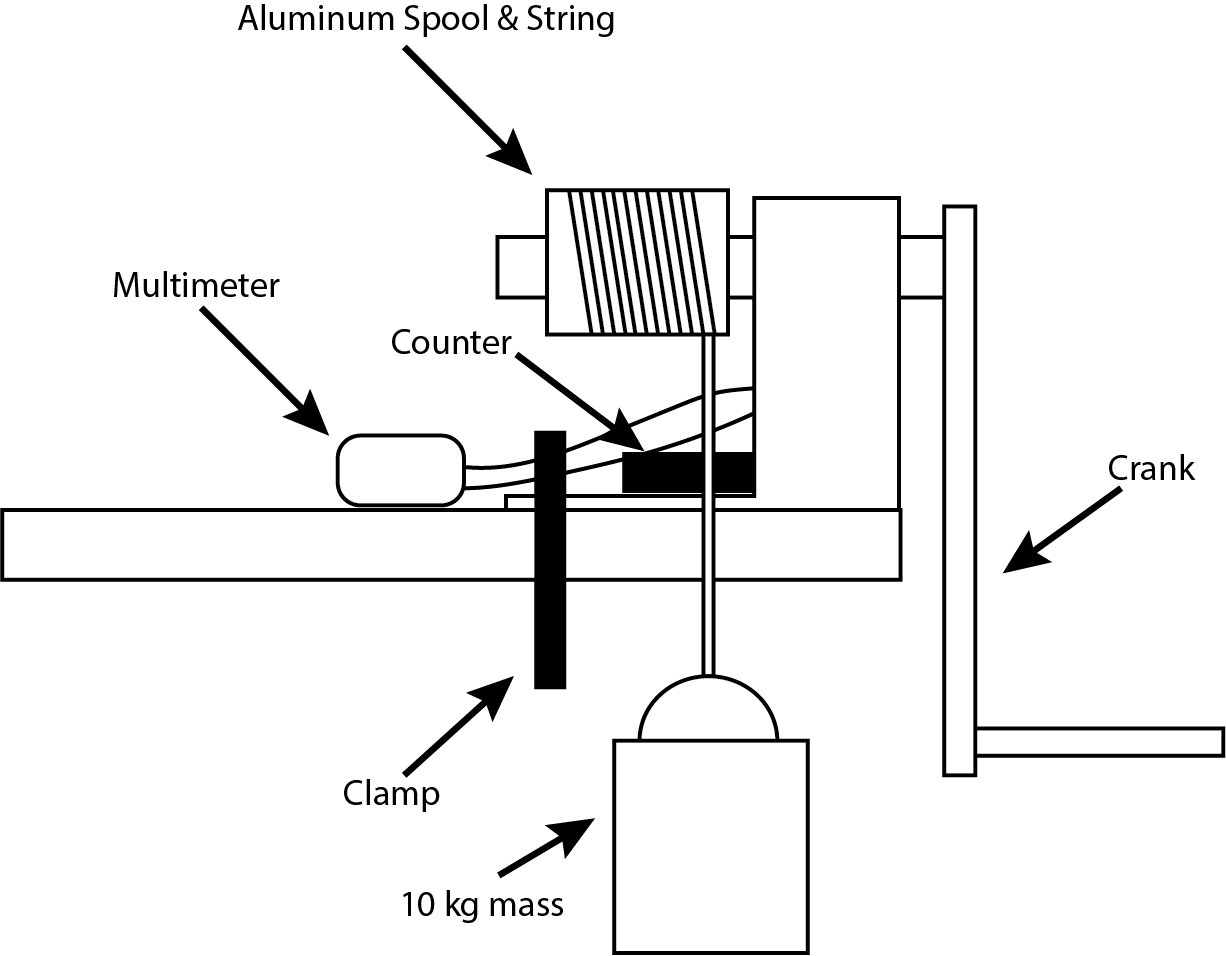
\includegraphics[width=0.9\linewidth]{4x/Asset 18@4x.png}
        \caption{Experimental Setup}
    \end{figure}
    \section{Data}
        \begin{center}
            \begin{tabular}{c|c|c|c|c|c}
                & \(m\) (g) & \(M\) (g) & \(D_1\) (cm) & \(D_2\) (cm) & N\\
                \hline
                1 & 200.53 & 305.31 & 4.785 & 4.918 & 186\\
                2 & 200.56 & 305.28 & 4.778 & 4.922 & \\
                3 & 200.60 & 305.25 & 4.779 & 4.898 & \\
                \hline
                \(\overline{x}\) & 200.563 & 305.280 & 4.781 & 4.913\\
                \(\sigma_x\) & 0.0038 & 0.013 & 0.035 & 0.030
            \end{tabular}\\[6pt]
            Table 1: Apparatus measurements.\\[12pt]
        \end{center}
        \begin{center}
            \begin{tabular}{c|c|c|c|c|c|c|c|c}
                \(R_0\) (\(\mathrm{\Omega}\))  & \(T_0\) (\(\cel\)) & \(R_i\) (\(\mathrm{\Omega}\))  & \(T_i\) (\(\cel\)) & \(R_f\) (\(\mathrm{\Omega}\))  & \(T_f\) (\(\cel\)) & \(R_{f,exp}\) (\(\mathrm{\Omega}\))  & \(T_{f,exp}\) (\(\cel\))\\
                \hline
                114500 & 22.129 & 145680 & 17.129 & 90595 & 27.129 & 896000 & 27.339
            \end{tabular}
            Table 2: Spool temperature.\\
        \end{center}
    \section{Calculations}
        \begin{alignat*}{3}
            (1)~
            &&J&=\frac{W}{H}\\
            &&W&=\int \mathbf{F}\cdot d\mathbf{r} =\int \mathbf{\tau} \cdot d\mathbf{\theta}\\ 
            &&&=MgR\Delta\theta\\
            &&R&=\frac{\frac{D_1+D_2}{2}}{2}\\
            &&\Delta\theta&=2\pi N\\
            &&W&=\pi MgN\frac{D_1+D_2}{2}\\
            &&H&=mc(T_{f,exp}-T_i)\\
            &&c&=0.220 \units{cal/g\cel}\\
            &&J&=\frac{\pi MgN\frac{D_1+D_2}{2}}{(0.220 \units{cal/g\cel})m(T_{f,exp}-T_i)}\\\\
            (2)~
            &&J&=\frac{\pi (10.305280 \units{kg})(9.8 \units{m/s^2})(186)(0.04781 \units{m}+0.04913 \units{m})}{2(0.220 \units{cal/g\cel})(200.563 \units{g})(27.339 \units{\cel} - 17.129 \units{\cel})}\\
            &&&= 6.349 \units{J/cal}\\
            (3)~
            &&\frac{\sigma_{D1}}{D_1}&=\frac{0.035}{4.781}\\
            &&&=0.73\%\\
            &&\frac{\sigma_{D_2}}{D_2}&=\frac{0.030}{4.913}\\
            &&&=0.61\%\\
            &&\frac{\sigma_m}{m}&=\frac{0.0038}{200.563}\\
            &&&=0.0019\%\\
            &&\frac{\sigma_M}{M}&=\frac{0.013}{305.280}\\
            &&&=0.0043\%\\
            (4)~
            &&J_{D1}&=\frac{\pi (10.305280 \units{kg})(9.8 \units{m/s^2})(186)((0.04781+0.00035) \units{m}+0.04913 \units{m})}{2(0.220 \units{cal/g\cel})(200.563 \units{g})(27.339 \units{\cel} - 17.129 \units{\cel})}\\
            &&&=6.372\units{J/cal}\\
            &&J_{D2}&=\frac{\pi (10.305280 \units{kg})(9.8 \units{m/s^2})(186)(0.04781 \units{m}+(0.04913+0.00030 ) \units{m})}{2(0.220 \units{cal/g\cel})(200.563 \units{g})(27.339 \units{\cel} - 17.129 \units{\cel})}\\
            &&&=6.368\units{J/cal}\\
            &&\sigma_J &=\sqrt{(6.372\units{J/cal} - 6.349 \units{J/cal})^2+(6.368\units{J/cal}- 6.349 \units{J/cal})^2}\\
            &&&=0.030 \units{J/cal}
        \end{alignat*}
    \section{Conclusion}
        The conversion from calories to joules,\(J\), was found to be \((6.349 \pm 0.030 )\) J/cal. This is much higher than the expected value of \(4.186\) J/cal, which is not surprising because during the experiment, we were not able to keep the bucket at a consistent height, and it often fell to the ground, or we had to adjust the string. Both of these could change the number of turns required to heat the spool by changing the force that the string was exerting on it. Even after multiple attempts, we could not maintain a consistent height with the bucket. At one point the string also got wet because there was a hole in the plastic bag, but even after drying it, the bucket would still fall to the ground. This may have been just a matter of skill and with more practice we could have kept it aloft, but we ran out of class time to keep trying. Perhaps a different string exists that would have been more effective.
\end{document}